%---------------------------------------------------------------------------------------------------
%		storage.tex
%
%	This is file contains the storage measurements.
%
%	Author: Andrea Meneghinello
% Version: 0.1
%	Table of changes:
%		21/03/2016 -> document definition
%---------------------------------------------------------------------------------------------------
\section{Storage benchmark}
\label{sec:measurements-storage}
By means of Stream benchmark tool we want to measure the \acs{ram} performance of both virtualization
environments. In order to have a basis for comparison we initially have executed the tool on the native
machine and then in various interesting environments, including:

\begin{enumerate}
	\item{one Docker container over the native \acs{os};}
	\item{one \ac{kvm} \ac{vm};}
	\item{one Docker container inside one \ac{kvm} \ac{vm}.}
\end{enumerate}

Even if running a container inside a \ac{vm} creates a double layer of virtualization, we also evaluated
this scenario because this is the only available solution if we choose a \ac{iaas} (like \ac{aws}) instead
a \ac{paas} provider.

The \acs{ram} tests were performed twice. The first time they were executed with a configuration so that
the L2-cache was exceeded. Instead, in the last one they were executed with a configuration so that the
L3-cache was exceeded.

\subsection{Stream benchmark}
\label{sec:measurements-storage-stream}
The Stream benchmark \cite{streamBenchmark} is a synthetic benchmark program that measures sustainable
memory bandwidth when performing simple operation on vectors. Performance is dominated by the memory
bandwidth of the system with the working set engineered to be significantly larger than the available
caches. The main determinants of performance are the bandwidth to main memory, and to a much lesser
extent, the cost of handling \ac{tlb} misses. The memory access pattern is regular and the hardware
pre-fetchers typically latch on to the access pattern and pre-fetch data before it is needed. Performance
is therefore gated by memory bandwidth and not by latency.

The intent of Stream is not to suggest that ``real'' applications have no data re-use, but rather to
decouple the measurement of the memory subsystem from the hypothetical ``peak'' performance of the machine.
In this respect the test is quite complementary to the Linpack benchmark test, which is typically optimized
to the point that a very large fraction of full speed is obtained on modern machines, independent of the
performance of their memory systems.

The benchmark has four components and each one adds independent information to the final results. They are:

\begin{itemize}
	\item{\keyword{\textsc{copy}}: measures transfer rates in the absence of arithmetic operations;}
	\item{\keyword{\textsc{scale}}: adds a simple arithmetic operation on the array's elements;}
	\item{\keyword{\textsc{sum}}: adds a third operand to allow multiple load/store operations;}
	\item{\keyword{\textsc{triad}}: allows chained/overlapped/fused multiply/add operations.}
\end{itemize}

Table \ref{tbl:measurements-storage-stream} gives a summary on the operations performed during the entire
execution. The different components are executed in sequence one after the other.

\begin{center}
	\begin{tabular}{| l | p{3cm} | >{\centering}m{2.5cm} | c |}
		\hline
		\textit{Name} & \textit{Operation}       & \textit{Bytes per iteration} & \textit{\acs{flops} per iteration} \\ \hline
		Copy          & $a[i] = b[i]$            & 16                           & 0                                  \\ \hline
		Scale         & $a[i] = q * b[i]$        & 16                           & 1                                  \\ \hline
		Sum           & $a[i] = b[i] + c[i]$     & 24                           & 1                                  \\ \hline
		Triad         & $a[i] = b[i] + q * c[i]$ & 24                           & 2                                  \\ \hline
	\end{tabular}
	\captionof{table}{Operation performed by Stream benchmark.}
	\label{tbl:measurements-storage-stream}
\end{center}
 
STREAM dates back to a time when floating-point arithmetic was comparable in cost to memory accesses,
so that the copy test was significantly faster than the others. This is no longer the case on any machines
of interest to \ac{hpc}, and the four Stream bandwidth values are typically quite close to each other.

\subsection{Configuration}
\label{sec:measurements-storage-configuration}
The only necessary parameter for this benchmark is the array size. To find out the correct value
in order to exceed only the L2-cache and then the L3-cache we use the following formula:

\begin{center}
	\begin{equation}
		\frac{availableCache * 1024 * 4}{8} * availableCore
	\end{equation}
\end{center}

This drives us to build an array of $16\,777\,216$ elements to exceed the L2 cache and an array of
$167\,772\,160$ elements to exceed the L3 cache.

Source code was compiled with the ``gcc'' compiler using the OpenMP directives to exploit all the
available processors.

\subsection{Results}
\label{sec:measurements-storage-results}
After executing the test in the environments described in Section \ref{sec:measurements-storage} with
the configuration described in Section \ref{sec:measurements-storage-configuration} we collected the
execution time and the sustainable memory bandwidth for each listed environments.
Tables \ref{tbl:measurements-storage-results-native}, \ref{tbl:measurements-storage-results-docker},
\ref{tbl:measurements-storage-results-kvm} and \ref{tbl:measurements-storage-results-combo} contain
the collected results about the sustainable memory bandwidth and the execution time. Charts in Figures 
\ref{img:measurements-storage-results-l2Capacity} and \ref{img:measurements-storage-results-l3Capacity}
show the available bandwidth when L2 and L3-cache are respectively exceeded by the test. Instead charts
in Figures  \ref{img:measurements-storage-results-l2Time} and \ref{img:measurements-storage-results-l3Time}
show the access time to the main memory in both test environments.

\begin{center}
	\begin{tabular}{| l | l | r | r | r | r |}
		\hline
		\multicolumn{6}{| c |}{\textbf{Native }}                                                                                                                  \\ \hline
		\multirow{2}{*}{\textit{Type}} & \multirow{2}{*}{\textit{Operation}} & \multirow{2}{*}{\textit{Rate (MB/s)}} &  \multicolumn{3}{c |}{\textit{Time (s)}}   \\ \cline{4-6}
		                               &                                     &                                       & \textit{Min} & \textit{Max} & \textit{Avg} \\ \hline
		\multirow{4}{*}{L2 overflow}   & \textit{copy}                       & $25\,290.8915$                        & $0.0106$     & $0.0145$     & $0.0128$     \\ \cline{2-6}
		                               & \textit{scale}                      & $21\,804.5532$                        & $0.0123$     & $0,0205$     & $0.0144$     \\ \cline{2-6}
		                               & \textit{add}                        & $23\,243.8253$                        & $0.0173$     & $0.0225$     & $0.0191$     \\ \cline{2-6}
		                               & \textit{triad}                      & $23\,930.1989$                        & $0.0168$     & $0.0213$     & $0.0185$     \\ \hline
		\multirow{4}{*}{L3 overflow}   & \textit{copy}                       & $34\,888.0418$                        & $0.0769$     & $0.0807$     & $0.0779$     \\ \cline{2-6}
		                               & \textit{scale}                      & $35\,002.6863$                        & $0.0783$     & $0.0816$     & $0.0783$     \\ \cline{2-6}
		                               & \textit{add}                        & $39\,904.2086$                        & $0.1009$     & $0.1031$     & $0.1013$     \\ \cline{2-6}
		                               & \textit{triad}                      & $39\,946.1155$                        & $0.1008$     & $0.1031$     & $0.1026$     \\ \hline
	\end{tabular}
	\captionof{table}{Resume of benchmark on native}
	\label{tbl:measurements-storage-results-native}
\end{center}

\begin{center}
	\begin{tabular}{| l | l | r | r | r | r |}
		\hline
		\multicolumn{6}{| c |}{\textbf{Docker }}                                                                                                                  \\ \hline
		\multirow{2}{*}{\textit{Type}} & \multirow{2}{*}{\textit{Operation}} & \multirow{2}{*}{\textit{Rate (MB/s)}} &  \multicolumn{3}{c |}{\textit{Time (s)}}   \\ \cline{4-6}
		                               &                                     &                                       & \textit{Min} & \textit{Max} & \textit{Avg} \\ \hline
		\multirow{4}{*}{L2 overflow}   & \textit{copy}                       & $17\,957.7955$                        & $0.0149$     & $0.0196$     & $0.0176$     \\ \cline{2-6}
		                               & \textit{scale}                      & $18\,157.0402$                        & $0.0148$     & $0.0219$     & $0.0183$     \\ \cline{2-6}
		                               & \textit{add}                        & $18\,965.3995$                        & $0.0212$     & $0.0271$     & $0.0239$     \\ \cline{2-6}
		                               & \textit{triad}                      & $19\,480.1359$                        & $0.0207$     & $0.0284$     & $0.0241$     \\ \hline
		\multirow{4}{*}{L3 overflow}   & \textit{copy}                       & $34\,942.0707$                        & $0.0768$     & $0.0870$     & $0.0807$     \\ \cline{2-6}
		                               & \textit{scale}                      & $34\,577.0054$                        & $0.0776$     & $0.0949$     & $0.0847$     \\ \cline{2-6}
		                               & \textit{add}                        & $39\,856.8392$                        & $0.1010$     & $0.1227$     & $0.1084$     \\ \cline{2-6}
		                               & \textit{triad}                      & $39\,917.6961$                        & $0.1009$     & $0.1183$     & $0.1183$     \\ \hline
	\end{tabular}
	\captionof{table}{Resume of benchmark on Docker container}
	\label{tbl:measurements-storage-results-docker}
\end{center}

\begin{center}
	\begin{tabular}{| l | l | r | r | r | r |}
		\hline
		\multicolumn{6}{| c |}{\textbf{\ac{kvm} \ac{vm} }}                                                                                                        \\ \hline
		\multirow{2}{*}{\textit{Type}} & \multirow{2}{*}{\textit{Operation}} & \multirow{2}{*}{\textit{Rate (MB/s)}} &  \multicolumn{3}{c |}{\textit{Time (s)}}   \\ \cline{4-6}
		                               &                                     &                                       & \textit{Min} & \textit{Max} & \textit{Avg} \\ \hline
		\multirow{4}{*}{L2 overflow}   & \textit{copy}                       & $16\,728.0764$                        & $0.0160$     & $0.0232$     & $0.0203$     \\ \cline{2-6}
		                               & \textit{scale}                      & $14\,775.9771$                        & $0.0182$     & $0.0238$     & $0.0199$     \\ \cline{2-6}
		                               & \textit{add}                        & $15\,341.6046$                        & $0.0262$     & $0.0311$     & $0.0282$     \\ \cline{2-6}
		                               & \textit{triad}                      & $18\,268.3036$                        & $0.0220$     & $0.0310$     & $0.0270$     \\ \hline
		\multirow{4}{*}{L3 overflow}   & \textit{copy}                       & $34\,942.0707$                        & $0.1325$     & $0.1768$     & $0.1549$     \\ \cline{2-6}
		                               & \textit{scale}                      & $34\,577.0054$                        & $0.1390$     & $0.1606$     & $0.1518$     \\ \cline{2-6}
		                               & \textit{add}                        & $39\,856.8392$                        & $0.1827$     & $0.2428$     & $0.2011$     \\ \cline{2-6}
		                               & \textit{triad}                      & $39\,917.6961$                        & $0.1751$     & $0.2066$     & $0.1965$     \\ \hline
	\end{tabular}
	\captionof{table}{Resume of benchmark on \acs{kvm} \acs{vm}}
	\label{tbl:measurements-storage-results-kvm}
\end{center}

\begin{center}
	\begin{tabular}{| l | l | r | r | r | r |}
		\hline
		\multicolumn{6}{| c |}{\textbf{Docker container inside a \ac{kvm} \ac{vm}}}                                                                               \\ \hline
		\multirow{2}{*}{\textit{Type}} & \multirow{2}{*}{\textit{Operation}} & \multirow{2}{*}{\textit{Rate (MB/s)}} &  \multicolumn{3}{c |}{\textit{Time (s)}}   \\ \cline{4-6}
		                               &                                     &                                       & \textit{Min} & \textit{Max} & \textit{Avg} \\ \hline
		\multirow{4}{*}{L2 overflow}   & \textit{copy}                       & $17\,025.0394$                        & $0.0158$     & $0.0283$     & $0.0192$     \\ \cline{2-6}
		                               & \textit{scale}                      & $16\,022.2554$                        & $0.0168$     & $0.0314$     & $0.0205$     \\ \cline{2-6}
		                               & \textit{add}                        & $21\,185.5672$                        & $0.0190$     & $0.0369$     & $0.0251$     \\ \cline{2-6}
		                               & \textit{triad}                      & $20\,452.8098$                        & $0.0197$     & $0.0391$     & $0.0243$     \\ \hline
		\multirow{4}{*}{L3 overflow}   & \textit{copy}                       & $17\,133.2818$                        & $0.1567$     & $0.1975$     & $0.1701$     \\ \cline{2-6}
		                               & \textit{scale}                      & $20\,331.0000$                        & $0.1320$     & $0.2177$     & $0.1641$     \\ \cline{2-6}
		                               & \textit{add}                        & $23\,684.9061$                        & $0.1700$     & $0.2359$     & $0.2074$     \\ \cline{2-6}
		                               & \textit{triad}                      & $20\,177.8757$                        & $0.1996$     & $0.2393$     & $0.2197$     \\ \hline
	\end{tabular}
	\captionof{table}{Resume of benchmark on a container inside a \acs{kvm} \acs{vm}}
	\label{tbl:measurements-storage-results-combo}
\end{center}

From charts \ref{img:measurements-storage-results-l3Capacity} and \ref{img:measurements-storage-results-l3Time}
we can assert that the \acs{os}-level virtualization provided by Docker containers is able to access
to the main memory almost in the same time of the native execution and it is able to exploit completely
the available bandwidth. Instead the hardware-level virtualization, provided by \ac{kvm} splits in half
the bandwidth and doubles the access time to the main memory. This is due to the overhead introduced by
hypervisor.

\begin{figure}
	\centering{}
	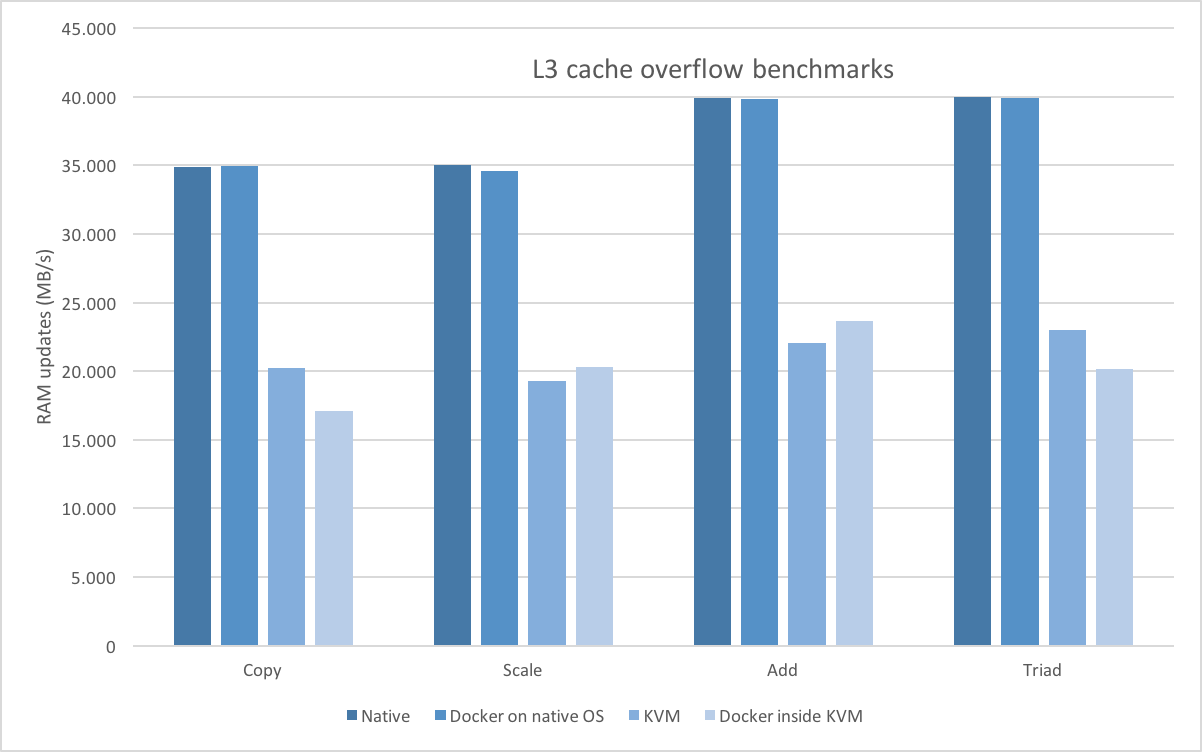
\includegraphics[width=0.8\textwidth]{chapters/measurements/images/storage-l3-capacity.png}
	\caption[Storage - overflow L3 cache]{Resume of benchmark when the L3 cache is exceeded}
	\label{img:measurements-storage-results-l3Capacity}
\end{figure}

Also in this case executing a Docker container inside a \ac{kvm} \ac{vm} do not produce a substantial
downgrade of the performance with respect to the execution without Docker in the \ac{vm}. Also in this
scenario we have demonstrated that the \acs{os}-level virtualization layer is not officious.

\begin{figure}
	\centering{}
	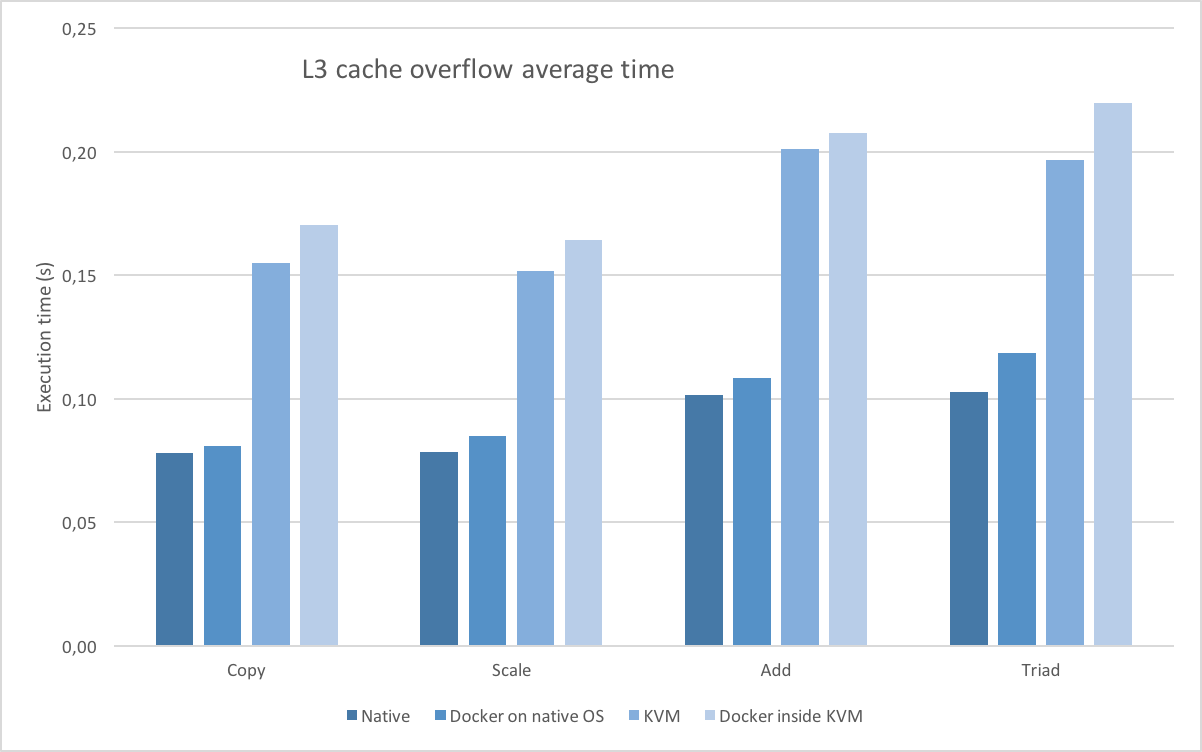
\includegraphics[width=0.8\textwidth]{chapters/measurements/images/storage-l3-time.png}
	\caption[Storage - access time L2 cache exceeded]{Resume of memory access time when the L2
		cache is exceeded.}
	\label{img:measurements-storage-results-l3Time}
\end{figure}

Instead, analysing charts illustrated in Figure \ref{img:measurements-storage-results-l2Capacity}
and \ref{img:measurements-storage-results-l2Time} when only L2 cache is exceeded the performance are
downgraded almost in the same way in all the tested scenarios regard to native execution. This is
imputable to the position of data in the caches associated to each core.

\begin{figure}
	\centering{}
	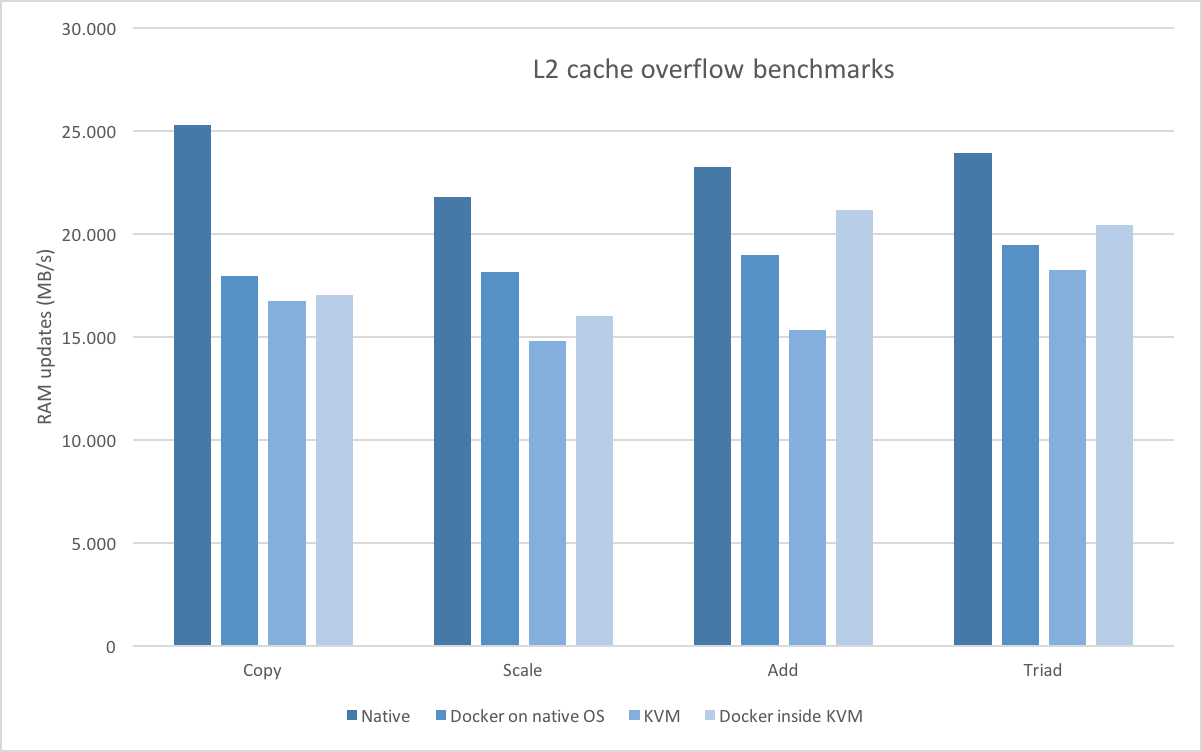
\includegraphics[width=0.8\textwidth]{chapters/measurements/images/storage-l2-capacity.png}
	\caption[Storage - overflow L2 cache]{Resume of benchmark when the L2 cache is exceeded}
	\label{img:measurements-storage-results-l2Capacity}
\end{figure}

\begin{figure}
	\centering{}
	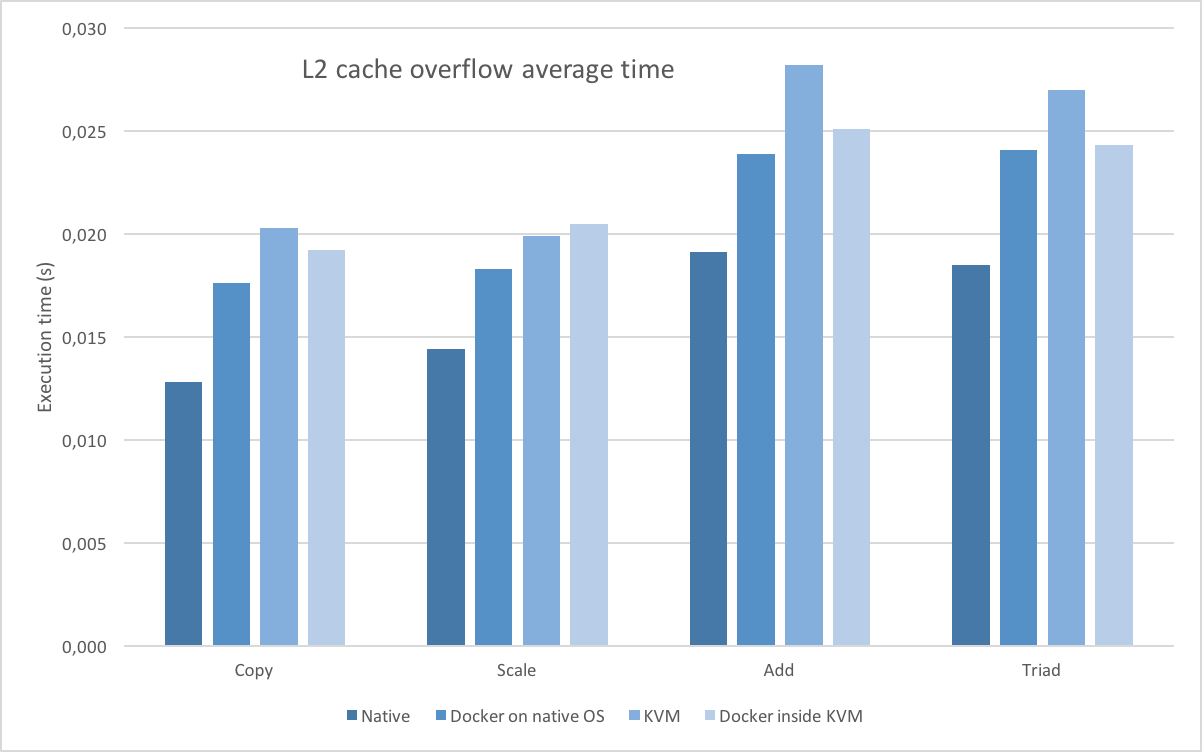
\includegraphics[width=0.8\textwidth]{chapters/measurements/images/storage-l2-time.png}
	\caption[Storage - access time L2 cache exceeded]{Resume of memory access time when the L2
		cache is exceeded.}
	\label{img:measurements-storage-results-l2Time}
\end{figure}